\section{Wireframing}

A primeira fase de conceção da interface, consistiu na elaboração de \emph{Wireframes}, protótipos de baixa fidelidade, que tiveram como objetivos:

\begin{itemize}
	\item Identificar funcionalidades do sistema
	\item Identificar cenários complexos
	\item Compreensão de fluxos e processos
	\item Abtração das questões estéticas
\end{itemize}

Para além dos objetivos, houve a preocupação de saber a opinião de outras pessoas, que se enquadram no público alvo a quem se destina o \emph{BillMate}

Para a conceção de \emph{Wireframes}, recorreu-se à aplicação \emph{Web} \emph{Moqups}. Na figura ~\ref{fig:mockup_dashboard} está representado o \emph{Wireframe} correspondente à \emph{Dashboard} quando acedida a partir de um \emph{browser}. Sendo esta a página mais importante da aplicação, houve um cuidado em aplicar ao máximo padrões sobre interfaces. Os padrões que mais se destacam são:

\begin{itemize}
	\item \emph{Dashboard}
	\item \emph{Accordions}
	\item \emph{Modals}
\end{itemize}

\begin{figure}[ht]
\centering
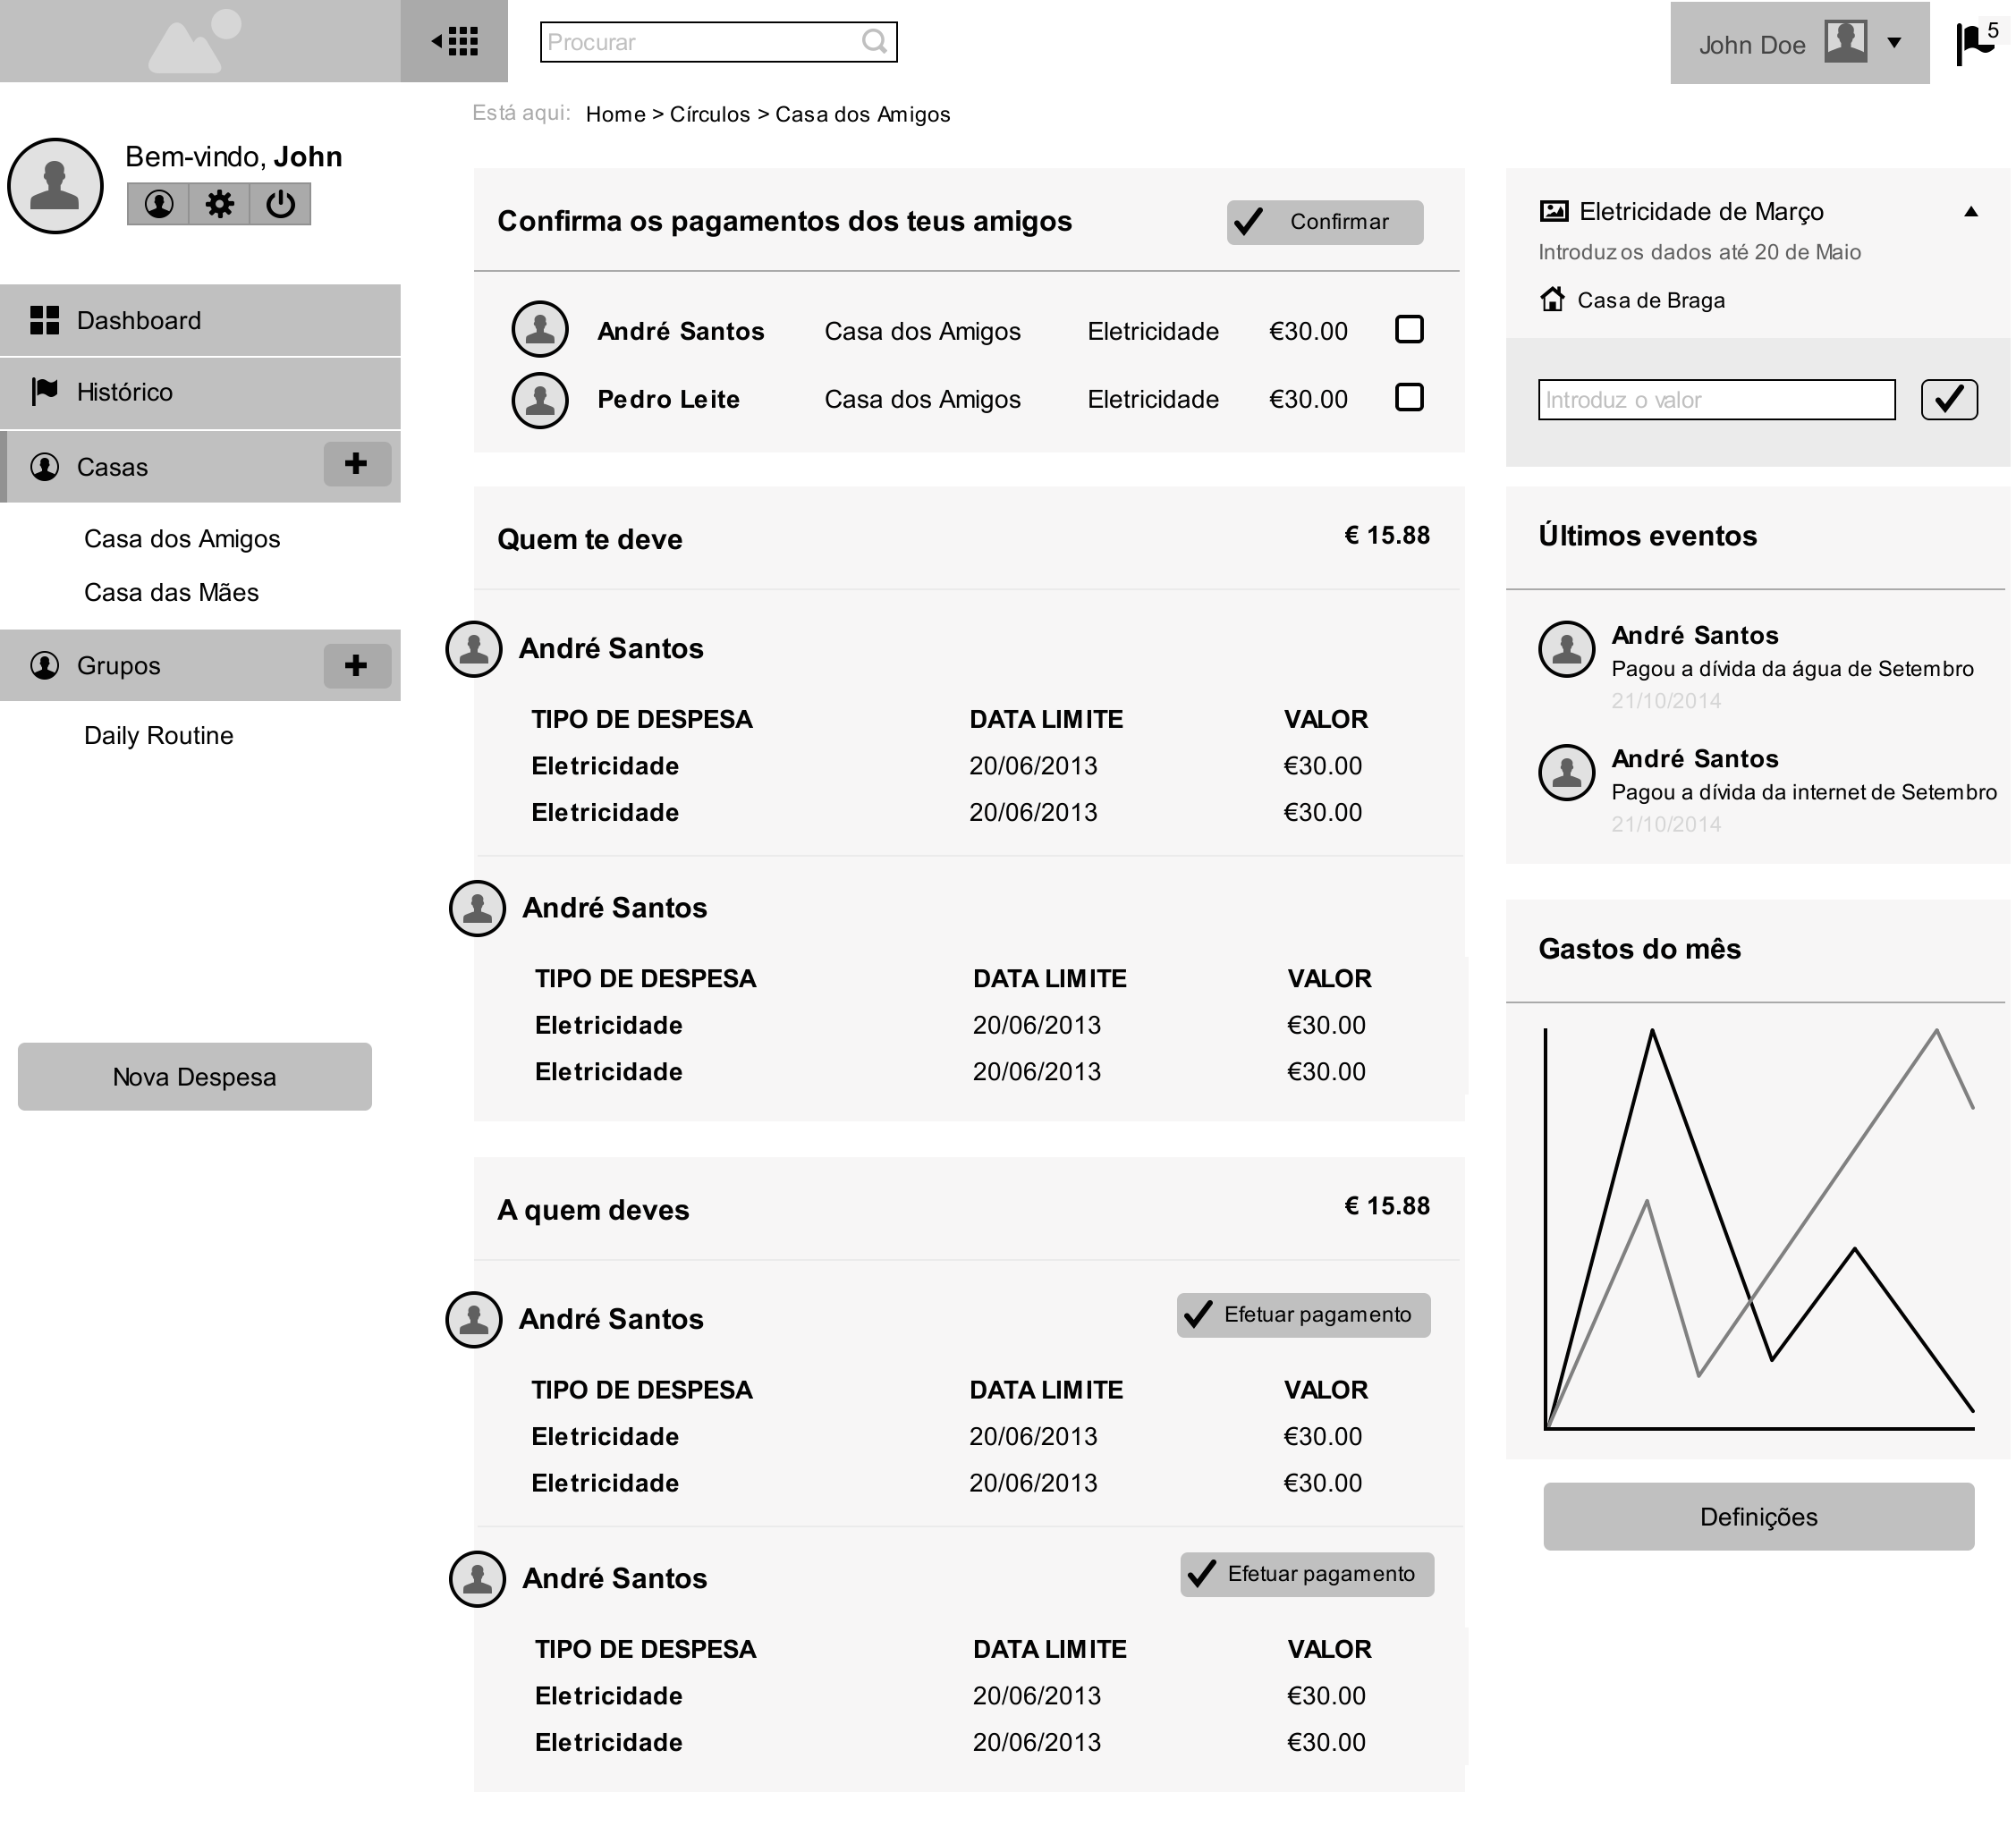
\includegraphics[width=.9\textwidth]{images/mockup_dashboard}
\caption{Dashboard vista a partir de um \emph{browser}}
\label{fig:mockup_dashboard}
\end{figure}

Nesta mesma fase, houve a preocupação de conceber a aplicação para outros equipamentos e que esta se adapta-se à ecrãs de diferentes tamanhos.

Na figura ~\ref{fig:mockup_mobile} está o \emph{Wireframe} correspondente à \emph{Dashboard} quando acedida a partir da aplicação \emph{mobile}. Nesta aplicação, as principais preocupações foram:

\begin{itemize}
	\item Mater a semelhança com a aplicação \emph{Web},
	\item Reaproveitar a barra lateral para organizar conteúdo sob a forma de lista (como é o caso das casas e dos grupos)
	\item Converter modais em novas janelas
	\item As funcionailidades principais passam a estar disponiveis numa barra de navegação no fundo da página
\end{itemize}

\begin{figure}[ht]
\centering
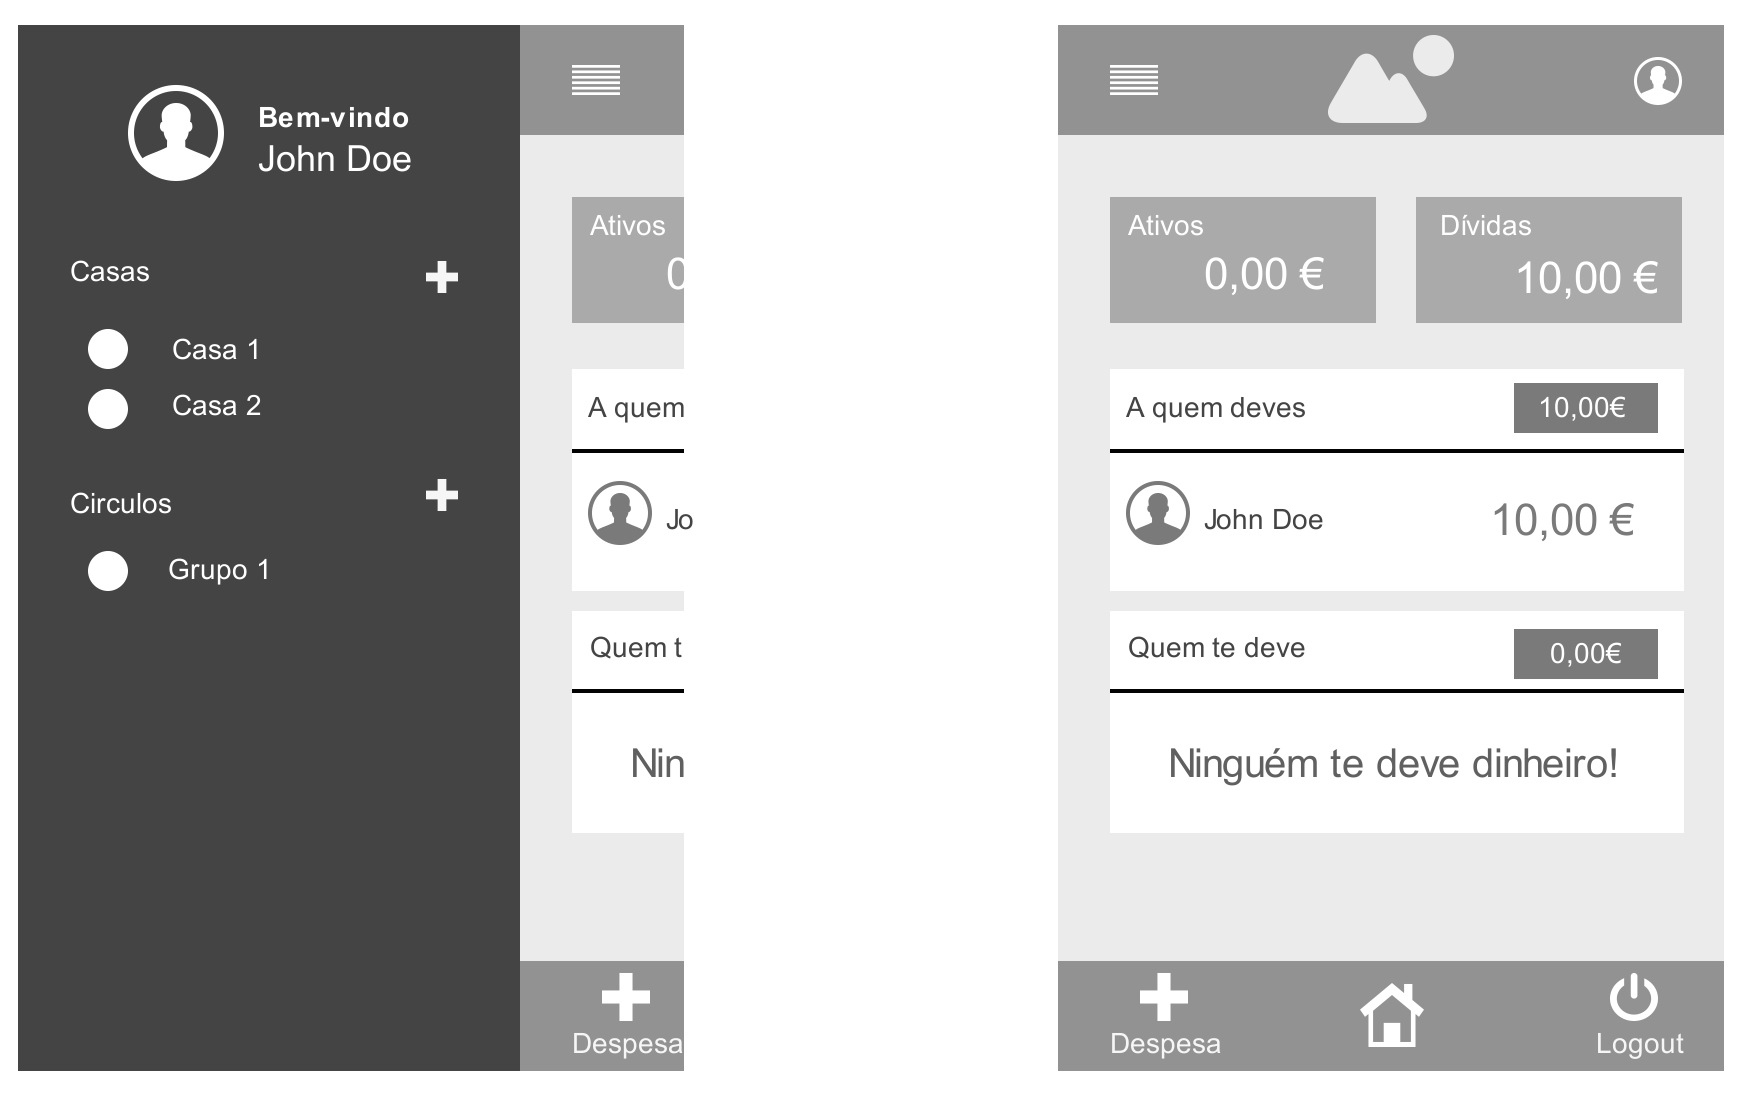
\includegraphics[width=.9\textwidth]{images/mobilemockup}
\caption{Dashboard vista a partir da aplicação \emph{mobile}}
\label{fig:mockup_mobile}
\end{figure}


